\documentclass[11pt]{article}

\usepackage[margin=1in]{geometry}
\usepackage[T1]{fontenc}
\usepackage[utf8]{inputenc}
\usepackage{lmodern}
\usepackage{amsmath,amssymb,amsthm,bm,mathtools}
\usepackage{booktabs}
\usepackage{array}
\usepackage{longtable}
\usepackage{graphicx}
\usepackage{caption}
\usepackage{subcaption}
\usepackage{xcolor}
\usepackage{hyperref}
\usepackage{enumitem}
\usepackage{listings}
\usepackage{float}

\hypersetup{
  colorlinks=true,
  linkcolor=blue!60!black,
  citecolor=blue!60!black,
  urlcolor=blue!60!black
}

\lstdefinestyle{pythonstyle}{
    language=Python,
    basicstyle=\ttfamily\small,
    keywordstyle=\color{blue!70!black},
    commentstyle=\color{green!40!black},
    stringstyle=\color{red!60!black},
    showstringspaces=false,
    breaklines=true,
    frame=single,
    rulecolor=\color{black!20},
    columns=fullflexible
}

\newtheorem{theorem}{Theorem}
\newtheorem{proposition}{Proposition}
\newtheorem{remark}{Remark}
\newtheorem{definition}{Definition}

\newcommand{\R}{\mathbb{R}}
\newcommand{\E}{\mathbb{E}}
\newcommand{\Var}{\operatorname{Var}}
\newcommand{\Cov}{\operatorname{Cov}}
\newcommand{\Normal}{\mathcal{N}}
\newcommand{\KL}{\operatorname{KL}}
\newcommand{\dint}{\,\mathrm{d}}

\title{From Gaussian AR(1) Belief Propagation to General Markov-Chain Diffusion Scores\\
\large Exact BP, continuous-message bottlenecks, and Gaussian-message approximation error}
\author{Prepared for the thesis project discussion}
\date{July 2026}

\begin{document}
\maketitle

\begin{abstract}
This note generalizes the Gaussian AR(1) belief-propagation derivation to arbitrary clean Markov-chain priors observed through coordinatewise Ornstein--Uhlenbeck noising. The main point is structural: Gaussianity is not needed for BP exactness. If the clean prior is a chain and the likelihood factorizes sitewise, then the posterior is again a chain, hence a tree factor graph, and sum-product BP computes exact posterior marginals. The diffusion score is then obtained from the exact identity
\[
  \nabla_{x_i}\log p_t(x) = -\frac{x_i-\alpha_t\E[a_i\mid x]}{\Delta_t}.
\]
Gaussianity only gives a finite-dimensional closure of the continuous BP messages. Outside the Gaussian case, messages are continuous probability functions and must be represented numerically or approximated. We therefore design two algorithms: reference grid BP, and Gaussian message closure carried out directly on the two information parameters. A proposition below shows that the latter is exactly the linear (LMMSE) denoiser, so the error it incurs is the excess error of the best linear estimator over the exact one. The grid is validated in the Gaussian AR(1) case against the exact precision-matrix score, and then used as a numerical proxy for the true score in a Laplace-innovation non-Gaussian chain. The experiments quantify the Gaussian-message approximation error at the posterior-mean and score levels.
\end{abstract}

\tableofcontents
\newpage

\section{Executive summary}

The Gaussian AR(1) calculation was useful, but it was not the most general statement. The correct general statement is:
\[
\boxed{\text{Markov clean prior} + \text{coordinatewise OU noising}
\Rightarrow \text{posterior chain}}
\]
so
\[
\boxed{\text{sum-product BP is exact, because chains are trees}.}
\]
Then the diffusion score follows from the posterior mean:
\[
\boxed{
  s_i(x,t) = \partial_{x_i}\log p_t(x)
  = -\frac{x_i-\alpha_t m_i(x,t)}{\Delta_t},
  \qquad m_i(x,t)=\E[a_i\mid x].
}
\]

The conceptual difference between the Gaussian and non-Gaussian cases is not exactness. The difference is representation:
\begin{center}
\begin{tabular}{lll}
\toprule
Case & BP exact? & Message representation \\
\midrule
Gaussian AR(1) & yes & two scalars: precision and information \\
Finite-state Markov chain & yes & finite vector \\
Continuous non-Gaussian Markov chain & yes & full function/density \\
\bottomrule
\end{tabular}
\end{center}

Therefore the computational problem is:
\[
\boxed{\text{In continuous non-Gaussian chains, exact BP propagates functions.}}
\]
The Gaussian-message approximation forces those functions to remain Gaussian. Jerome's question is then naturally formalized as:
\[
\boxed{\text{How large is the error caused by Gaussian message closure?}}
\]

The code implements the following experimental pipeline:
\begin{enumerate}[label=\arabic*.]
  \item Validate grid BP in the Gaussian AR(1) case, where the exact score is known by linear algebra.
  \item In a Laplace-innovation AR(1) chain, estimate grid discretization error by comparing a coarse grid with a fine grid.
  \item In the same Laplace chain, compare Gaussian message closure with reference grid BP.
  \item Convert all posterior-mean errors into score errors using the exact OU identity.
\end{enumerate}

\section{The diffusion setup}

\subsection{Clean chain prior}

Let
\[
  a_{1:n}=(a_1,\ldots,a_n)
\]
be clean latent variables. For now take each
\[
  a_i\in\mathcal A\subseteq \R,
\]
but the same factorization logic works for finite state spaces, vector-valued states, or mixed spaces with the appropriate sums/integrals.

The clean prior is assumed to be Markov along the sequence index:
\begin{equation}
  p_0(a_{1:n})
  = \mu(a_1)\prod_{i=2}^n K_i(a_i\mid a_{i-1}),
  \label{eq:markov-prior}
\end{equation}
where \(\mu\) is the initial density and \(K_i\) is a transition density or kernel.

This is the structural assumption. It does not assume Gaussianity. For example, \(K_i\) can be Gaussian, Laplace, mixture Gaussian, nonlinear, bounded-support, or discrete.

\subsection{Coordinatewise OU noising}

At diffusion time \(t>0\), we observe
\begin{equation}
  x_i = \alpha_t a_i + \sqrt{\Delta_t}\,z_i,
  \qquad z_i\sim \Normal(0,1),
  \label{eq:ou-noising}
\end{equation}
independently over \(i\), with
\begin{equation}
  \alpha_t=e^{-t},
  \qquad
  \Delta_t=1-e^{-2t}=1-\alpha_t^2.
  \label{eq:alpha-delta}
\end{equation}
The one-site likelihood is therefore
\begin{equation}
  \ell_i(a_i;x_i)
  := p_t(x_i\mid a_i)
  = \Normal(x_i;\alpha_t a_i,\Delta_t).
  \label{eq:likelihood}
\end{equation}
Written explicitly,
\begin{equation}
  \ell_i(a_i;x_i)
  = \frac{1}{\sqrt{2\pi\Delta_t}}
  \exp\left[-\frac{(x_i-\alpha_t a_i)^2}{2\Delta_t}\right].
  \label{eq:likelihood-explicit}
\end{equation}
Because the noises \(z_i\) are independent, the full likelihood factorizes:
\begin{equation}
  p_t(x_{1:n}\mid a_{1:n})
  = \prod_{i=1}^n \ell_i(a_i;x_i).
  \label{eq:factorized-likelihood}
\end{equation}

\section{Posterior factorization: the posterior remains a chain}

\begin{proposition}[Posterior chain factorization]
Assume the clean prior has the Markov factorization \eqref{eq:markov-prior} and the likelihood factorizes as in \eqref{eq:factorized-likelihood}. Then the posterior is
\begin{equation}
  p_t(a_{1:n}\mid x_{1:n})
  = \frac{1}{Z_t(x)}
  \mu(a_1)
  \prod_{i=2}^n K_i(a_i\mid a_{i-1})
  \prod_{i=1}^n \ell_i(a_i;x_i),
  \label{eq:posterior-chain}
\end{equation}
where
\[
  Z_t(x)=p_t(x_{1:n})
\]
is the evidence. Hence the posterior factor graph is a chain with unary observation factors.
\end{proposition}

\begin{proof}
Start from Bayes' rule:
\begin{equation}
  p_t(a_{1:n}\mid x_{1:n})
  = \frac{p_0(a_{1:n})p_t(x_{1:n}\mid a_{1:n})}{p_t(x_{1:n})}.
\end{equation}
Now substitute the Markov prior:
\begin{equation}
  p_0(a_{1:n}) = \mu(a_1)\prod_{i=2}^n K_i(a_i\mid a_{i-1}),
\end{equation}
and the factorized likelihood:
\begin{equation}
  p_t(x_{1:n}\mid a_{1:n}) = \prod_{i=1}^n \ell_i(a_i;x_i).
\end{equation}
Therefore
\begin{align}
  p_t(a_{1:n}\mid x_{1:n})
  &= \frac{1}{p_t(x_{1:n})}
  \left[\mu(a_1)\prod_{i=2}^n K_i(a_i\mid a_{i-1})\right]
  \left[\prod_{i=1}^n \ell_i(a_i;x_i)\right] \\
  &= \frac{1}{Z_t(x)}
  \mu(a_1)
  \prod_{i=2}^n K_i(a_i\mid a_{i-1})
  \prod_{i=1}^n \ell_i(a_i;x_i).
\end{align}
Every transition factor touches only adjacent variables \((a_{i-1},a_i)\), and every likelihood factor touches only one variable \(a_i\). Thus no loops are created. The posterior graph is still a chain.\end{proof}

Graphically, the posterior structure is
\[
  a_1 - a_2 - \cdots - a_n,
\]
with one unary likelihood \(\ell_i\) attached to each \(a_i\). This is why the BP exactness argument applies.

\section{Generic sum-product BP and exactness on trees}

\subsection{Generic factor graph notation}

Let a distribution factorize as
\begin{equation}
  p(a) = \frac{1}{Z}\prod_{f\in F}\psi_f(a_{\partial f}),
  \label{eq:generic-factorization}
\end{equation}
where \(F\) is the set of factors and \(\partial f\) is the set of variables adjacent to factor \(f\). Let \(\partial i\) be the set of factors adjacent to variable \(a_i\).

Sum-product BP passes two types of messages.

The variable-to-factor message is
\begin{equation}
  m_{i\to f}(a_i)
  \propto
  \prod_{g\in \partial i\setminus f} m_{g\to i}(a_i).
  \label{eq:var-to-factor}
\end{equation}
The factor-to-variable message is
\begin{equation}
  m_{f\to i}(a_i)
  \propto
  \int
  \psi_f(a_{\partial f})
  \prod_{j\in \partial f\setminus i}m_{j\to f}(a_j)
  \prod_{j\in \partial f\setminus i}\mathrm{d}a_j.
  \label{eq:factor-to-var}
\end{equation}
For discrete variables, the integrals are replaced by sums.

Once messages have converged, or after the two sweeps on a tree, the belief at variable \(i\) is
\begin{equation}
  b_i(a_i)
  =
  \frac{\prod_{f\in\partial i}m_{f\to i}(a_i)}
  {\int \prod_{f\in\partial i}m_{f\to i}(u)\,\mathrm{d}u}.
  \label{eq:belief-generic}
\end{equation}

\subsection{Why BP is exact on trees}

On a tree, deleting one edge separates the graph into two disconnected components. Therefore a message sent across an edge can be interpreted exactly as the partial marginal contribution of the whole subtree behind that edge.

For example, suppose a message is sent from a factor-side subtree to a boundary variable \(a_i\). The factor-to-variable update integrates all variables inside that subtree except the boundary variable. Since no loop reconnects that subtree to the rest of the graph, this partial marginal contribution is exact. When all incoming messages arrive at \(a_i\), multiplying them combines disjoint subtrees around \(a_i\). Normalizing gives the exact marginal.

Thus on a tree factor graph,
\begin{equation}
  b_i(a_i)=p(a_i)
  \label{eq:bp-exact-tree}
\end{equation}
exactly. Since a chain is connected and acyclic, a chain is a tree.

\begin{remark}
The reason BP is exact here is the Markov-chain structure of the clean prior over the sequence index plus independent sitewise noising. It is not merely the fact that the forward diffusion process is Markov in diffusion time. Diffusion-time Markovianity and sequence-index Markovianity are different statements.
\end{remark}

\section{Forward-backward BP for the posterior chain}

For the chain posterior \eqref{eq:posterior-chain}, generic BP becomes the forward-backward algorithm.

Define left messages \(L_i\) and right messages \(R_i\) so that the local likelihood \(\ell_i\) is kept outside the incoming message at site \(i\). Initialize
\begin{equation}
  L_1(a_1)=\mu(a_1),
  \qquad
  R_n(a_n)=1.
\end{equation}
Then for \(i=1,\ldots,n-1\),
\begin{equation}
  L_{i+1}(a_{i+1})
  =
  \int_{\mathcal A}
  K_{i+1}(a_{i+1}\mid a_i)
  L_i(a_i)\ell_i(a_i;x_i)
  \mathrm{d}a_i.
  \label{eq:left-message}
\end{equation}
For \(i=n,n-1,\ldots,2\),
\begin{equation}
  R_{i-1}(a_{i-1})
  =
  \int_{\mathcal A}
  K_i(a_i\mid a_{i-1})
  R_i(a_i)\ell_i(a_i;x_i)
  \mathrm{d}a_i.
  \label{eq:right-message}
\end{equation}

The posterior belief at site \(i\) is
\begin{equation}
  b_i(a_i)
  =
  \frac{L_i(a_i)\ell_i(a_i;x_i)R_i(a_i)}
  {\int_{\mathcal A} L_i(u)\ell_i(u;x_i)R_i(u)\,\mathrm{d}u}.
  \label{eq:chain-belief}
\end{equation}
Because the posterior graph is a chain,
\begin{equation}
  b_i(a_i)=p_t(a_i\mid x_{1:n}).
  \label{eq:belief-exact}
\end{equation}
Therefore the exact posterior mean is
\begin{equation}
  m_i(x,t)
  := \E_t[a_i\mid x_{1:n}]
  = \int_{\mathcal A} a_i b_i(a_i)\,\mathrm{d}a_i.
  \label{eq:posterior-mean}
\end{equation}

\section{The score identity: every algebraic step}

This is the key diffusion-specific identity. The noisy marginal is
\begin{equation}
  p_t(x_{1:n})
  = \int_{\mathcal A^n}
  p_0(a_{1:n})
  \prod_{j=1}^n \Normal(x_j;\alpha_t a_j,\Delta_t)
  \mathrm{d}a_{1:n}.
  \label{eq:noisy-marginal}
\end{equation}
For compact notation define
\begin{equation}
  g_j(x_j\mid a_j)
  := \Normal(x_j;\alpha_t a_j,\Delta_t).
\end{equation}
Then
\begin{equation}
  p_t(x) = \int p_0(a)\prod_{j=1}^n g_j(x_j\mid a_j)\,\mathrm{d}a.
\end{equation}

We compute the \(i\)-th score component:
\begin{equation}
  s_i(x,t)=\partial_{x_i}\log p_t(x).
\end{equation}
Using
\begin{equation}
  \partial_{x_i}\log p_t(x)=\frac{\partial_{x_i}p_t(x)}{p_t(x)},
  \label{eq:log-derivative}
\end{equation}
we first differentiate the marginal density. Under the usual regularity/dominated-convergence conditions that hold for the Gaussian likelihoods used here,
\begin{align}
  \partial_{x_i}p_t(x)
  &= \partial_{x_i}\int p_0(a)\prod_{j=1}^n g_j(x_j\mid a_j)\,\mathrm{d}a \\
  &= \int p_0(a)\partial_{x_i}\left[\prod_{j=1}^n g_j(x_j\mid a_j)\right]\,\mathrm{d}a.
  \label{eq:diff-under-integral}
\end{align}
Only the factor \(g_i(x_i\mid a_i)\) depends on \(x_i\), so
\begin{equation}
  \partial_{x_i}\left[\prod_{j=1}^n g_j(x_j\mid a_j)\right]
  =
  \left[\partial_{x_i}g_i(x_i\mid a_i)\right]
  \prod_{j\ne i}g_j(x_j\mid a_j).
\end{equation}
Now compute the derivative of the Gaussian factor explicitly:
\begin{align}
  g_i(x_i\mid a_i)
  &= \frac{1}{\sqrt{2\pi\Delta_t}}
  \exp\left[-\frac{(x_i-\alpha_t a_i)^2}{2\Delta_t}\right],\\
  \log g_i(x_i\mid a_i)
  &= -\frac12\log(2\pi\Delta_t)
  -\frac{(x_i-\alpha_t a_i)^2}{2\Delta_t},\\
  \partial_{x_i}\log g_i(x_i\mid a_i)
  &= -\frac{1}{2\Delta_t}\partial_{x_i}(x_i-\alpha_t a_i)^2,\\
  &= -\frac{1}{2\Delta_t}\,2(x_i-\alpha_t a_i),\\
  &= -\frac{x_i-\alpha_t a_i}{\Delta_t}.
\end{align}
Therefore
\begin{equation}
  \partial_{x_i}g_i(x_i\mid a_i)
  = g_i(x_i\mid a_i)\partial_{x_i}\log g_i(x_i\mid a_i)
  = -\frac{x_i-\alpha_t a_i}{\Delta_t}g_i(x_i\mid a_i).
  \label{eq:gaussian-derivative}
\end{equation}
Substitute \eqref{eq:gaussian-derivative} into \eqref{eq:diff-under-integral}:
\begin{align}
  \partial_{x_i}p_t(x)
  &= \int p_0(a)
  \left[-\frac{x_i-\alpha_t a_i}{\Delta_t}g_i(x_i\mid a_i)\right]
  \prod_{j\ne i}g_j(x_j\mid a_j)
  \mathrm{d}a \\
  &= \int p_0(a)
  \prod_{j=1}^n g_j(x_j\mid a_j)
  \left[-\frac{x_i-\alpha_t a_i}{\Delta_t}\right]
  \mathrm{d}a.
  \label{eq:partial-marginal}
\end{align}
Divide by \(p_t(x)\):
\begin{align}
  \partial_{x_i}\log p_t(x)
  &= \frac{1}{p_t(x)}
  \int p_0(a)
  \prod_{j=1}^n g_j(x_j\mid a_j)
  \left[-\frac{x_i-\alpha_t a_i}{\Delta_t}\right]
  \mathrm{d}a.
\end{align}
Now use Bayes' rule in density form:
\begin{equation}
  p_t(a\mid x)
  = \frac{p_0(a)\prod_{j=1}^n g_j(x_j\mid a_j)}{p_t(x)}.
\end{equation}
Thus
\begin{align}
  \partial_{x_i}\log p_t(x)
  &= \int p_t(a\mid x)
  \left[-\frac{x_i-\alpha_t a_i}{\Delta_t}\right]
  \mathrm{d}a \\
  &= -\frac{1}{\Delta_t}
  \int p_t(a\mid x)(x_i-\alpha_t a_i)\,\mathrm{d}a \\
  &= -\frac{1}{\Delta_t}
  \left[
    x_i\int p_t(a\mid x)\,\mathrm{d}a
    -\alpha_t\int a_i p_t(a\mid x)\,\mathrm{d}a
  \right] \\
  &= -\frac{1}{\Delta_t}
  \left[x_i -\alpha_t\E_t[a_i\mid x]\right].
\end{align}
Therefore
\begin{equation}
  \boxed{
  s_i(x,t)
  = \partial_{x_i}\log p_t(x)
  = -\frac{x_i-\alpha_t m_i(x,t)}{\Delta_t},
  \qquad m_i(x,t)=\E_t[a_i\mid x].
  }
  \label{eq:score-identity}
\end{equation}

Combining \eqref{eq:belief-exact}, \eqref{eq:posterior-mean}, and \eqref{eq:score-identity} gives the main theorem.

\begin{theorem}[Exact score by BP for Markov-chain data under OU noising]
Assume
\[
  p_0(a_{1:n})=\mu(a_1)\prod_{i=2}^n K_i(a_i\mid a_{i-1})
\]
and
\[
  x_i=\alpha_t a_i+\sqrt{\Delta_t}z_i,
  \qquad z_i\sim\Normal(0,1)
\]
independently over \(i\). Then \(p_t(a_{1:n}\mid x_{1:n})\) is a chain-structured factor graph. Sum-product BP computes the exact posterior marginal
\[
  b_i(a_i)=p_t(a_i\mid x_{1:n}).
\]
If
\[
  m_i^{\rm BP}(x,t)=\int a_i b_i(a_i)\,\mathrm{d}a_i,
\]
then
\[
  m_i^{\rm BP}(x,t)=\E_t[a_i\mid x],
\]
and the exact diffusion score is
\begin{equation}
  \boxed{
  s_i(x,t)= -\frac{x_i-\alpha_t m_i^{\rm BP}(x,t)}{\Delta_t}.
  }
\end{equation}
In vector form,
\begin{equation}
  \boxed{
  \nabla_x\log p_t(x)=-\frac{x-\alpha_t m^{\rm BP}(x,t)}{\Delta_t}.
  }
\end{equation}
\end{theorem}

\section{What was special about the Gaussian AR(1) case?}

\subsection{Gaussian clean prior}

In the Gaussian AR(1) case,
\begin{equation}
  a_1\sim\Normal(0,1),
  \qquad
  a_i=\rho a_{i-1}+\sqrt{q}\,\xi_i,
  \qquad q=1-\rho^2,
\end{equation}
with \(\xi_i\sim\Normal(0,1)\). The transition is
\begin{equation}
  K_i(a_i\mid a_{i-1})=\Normal(a_i;\rho a_{i-1},q).
\end{equation}
The covariance matrix of the clean chain is
\begin{equation}
  \Sigma_0(i,j)=\rho^{|i-j|}.
\end{equation}
The noisy vector is also Gaussian:
\begin{equation}
  x=\alpha_t a+\sqrt{\Delta_t}z,
  \qquad
  a\sim\Normal(0,\Sigma_0),
  \qquad
  z\sim\Normal(0,I),
\end{equation}
so
\begin{equation}
  x\sim\Normal(0,\Sigma_t),
  \qquad
  \Sigma_t=\alpha_t^2\Sigma_0+\Delta_t I.
\end{equation}
For any centered Gaussian density
\[
  p(x)\propto \exp\left(-\frac12 x^\top\Sigma^{-1}x\right),
\]
we have
\begin{equation}
  \nabla_x\log p(x)=-\Sigma^{-1}x.
\end{equation}
Therefore the exact Gaussian score is
\begin{equation}
  \boxed{s_{\rm G}(x,t)=-\Sigma_t^{-1}x.}
  \label{eq:matrix-score}
\end{equation}
The exact Gaussian posterior mean is
\begin{equation}
  \boxed{m_{\rm G}(x,t)=\alpha_t\Sigma_0\Sigma_t^{-1}x.}
  \label{eq:gaussian-posterior-mean}
\end{equation}
One can verify directly that \eqref{eq:matrix-score} and \eqref{eq:score-identity} agree:
\begin{align}
  -\frac{x-\alpha_t m_{\rm G}}{\Delta_t}
  &= -\frac{x-\alpha_t(\alpha_t\Sigma_0\Sigma_t^{-1}x)}{\Delta_t}\\
  &= -\frac{[I-\alpha_t^2\Sigma_0\Sigma_t^{-1}]x}{\Delta_t}.
\end{align}
Since
\begin{equation}
  \Sigma_t=\alpha_t^2\Sigma_0+\Delta_t I,
\end{equation}
we have
\begin{equation}
  \Delta_t I=\Sigma_t-\alpha_t^2\Sigma_0.
\end{equation}
Multiplying on the right by \(\Sigma_t^{-1}\),
\begin{equation}
  \Delta_t\Sigma_t^{-1}=I-\alpha_t^2\Sigma_0\Sigma_t^{-1}.
\end{equation}
Hence
\begin{align}
  -\frac{[I-\alpha_t^2\Sigma_0\Sigma_t^{-1}]x}{\Delta_t}
  &= -\frac{\Delta_t\Sigma_t^{-1}x}{\Delta_t}\\
  &= -\Sigma_t^{-1}x.
\end{align}

\subsection{Gaussian message closure}
\label{sec:closureforms}

A Gaussian BP message can be written in information form as
\begin{equation}
  m(a)\propto \exp\left(-\frac12\lambda a^2+ha\right),
  \label{eq:gaussian-message}
\end{equation}
where \(\lambda\) is precision and \(h\) is information. Its mean and variance are
\begin{equation}
  \mu=\frac{h}{\lambda},
  \qquad
  v=\frac{1}{\lambda}.
\end{equation}

The OU likelihood as a function of \(a_i\) is also Gaussian-shaped:
\begin{align}
  \ell_i(a_i;x_i)
  &\propto
  \exp\left[-\frac{(x_i-\alpha_t a_i)^2}{2\Delta_t}\right]\\
  &\propto
  \exp\left[-\frac{\alpha_t^2}{2\Delta_t}a_i^2
  +\frac{\alpha_t x_i}{\Delta_t}a_i\right].
\end{align}
Thus multiplying a Gaussian message by the likelihood updates information parameters as
\begin{equation}
  \widetilde\lambda_i=\lambda_i+\frac{\alpha_t^2}{\Delta_t},
  \qquad
  \widetilde h_i=h_i+\frac{\alpha_t x_i}{\Delta_t}.
  \label{eq:likelihoodupdate}
\end{equation}
The resulting temporary mean and variance are
\begin{equation}
  \widetilde\mu_i=\frac{\widetilde h_i}{\widetilde\lambda_i},
  \qquad
  \widetilde v_i=\frac{1}{\widetilde\lambda_i}.
\end{equation}
Now apply the Gaussian transition
\begin{equation}
  a_{i+1}=\rho a_i+\sqrt q\xi_{i+1}.
\end{equation}
If \(a_i\) has temporary distribution \(\Normal(\widetilde\mu_i,\widetilde v_i)\), then
\begin{equation}
  a_{i+1}\sim\Normal(\rho\widetilde\mu_i, q+\rho^2\widetilde v_i).
\end{equation}
Therefore the outgoing left message remains Gaussian with
\begin{equation}
  \lambda_{i+1}=\frac{1}{q+\rho^2\widetilde v_i},
  \qquad
  h_{i+1}=\frac{\rho\widetilde\mu_i}{q+\rho^2\widetilde v_i}.
\end{equation}
This is the finite-dimensional closure. The message update is exact because products and marginalizations of Gaussian densities remain Gaussian.

\subsection{The key distinction}

The Gaussian AR(1) case combines two facts:
\begin{enumerate}[label=\arabic*.]
  \item BP is exact because the posterior graph is a chain.
  \item Messages are finite-dimensional because the Gaussian family is closed under the BP updates.
\end{enumerate}
The first fact survives for any Markov-chain prior. The second does not.

Therefore:
\[
\boxed{\text{Gaussianity gives closure, not exactness.}}
\]

\section{The continuous non-Gaussian bottleneck}

For a general continuous non-Gaussian transition \(K_i\), the update
\begin{equation}
  L_{i+1}(a_{i+1})
  =
  \int
  K_{i+1}(a_{i+1}\mid a_i)
  L_i(a_i)\ell_i(a_i;x_i)
  \mathrm{d}a_i
\end{equation}
maps one function into another function. Thus the message space is infinite-dimensional:
\begin{equation}
  L_i,R_i\in L^1_+(\R).
\end{equation}

This is the real computational issue. Exact BP exists mathematically, but one cannot store arbitrary functions exactly on a computer. We must approximate them.

The simplest hierarchy of approximations is:
\begin{center}
\begin{tabular}{lll}
\toprule
Approximation & Message representation & Comment \\
\midrule
Grid BP & values on \(M\) grid points & reference numerical method \\
Gaussian closure & mean and variance & tests Gaussian closure error \\
Gaussian mixture BP & mixture weights, means, variances & handles multimodality \\
Particle BP & weighted samples & Monte Carlo approximation \\
Basis expansion & coefficients in basis & Hermite/spline/Fourier style \\
Neural messages & amortized function/embedding & most flexible, but harder to justify \\
\bottomrule
\end{tabular}
\end{center}

In this project we focus first on the two cleanest algorithms: grid BP and Gaussian message closure.

\section{Approximation error and score error}

Let \(m_i(x,t)=\E[a_i\mid x]\) be the exact posterior mean and \(\widehat m_i(x,t)\) an approximation. Define
\begin{equation}
  s_i(x,t)=-\frac{x_i-\alpha_t m_i(x,t)}{\Delta_t},
  \qquad
  \widehat s_i(x,t)=-\frac{x_i-\alpha_t\widehat m_i(x,t)}{\Delta_t}.
\end{equation}
Then the score error is exactly
\begin{align}
  \widehat s_i-s_i
  &= -\frac{x_i-\alpha_t\widehat m_i}{\Delta_t}
  +\frac{x_i-\alpha_t m_i}{\Delta_t}\\
  &= \frac{-x_i+\alpha_t\widehat m_i+x_i-\alpha_t m_i}{\Delta_t}\\
  &= \frac{\alpha_t}{\Delta_t}(\widehat m_i-m_i).
\end{align}
Thus
\begin{equation}
  \boxed{
  \widehat s_i(x,t)-s_i(x,t)
  = \frac{\alpha_t}{\Delta_t}\left[\widehat m_i(x,t)-m_i(x,t)\right].
  }
  \label{eq:error-identity}
\end{equation}
This identity is important because it tells us that all approximation errors enter through posterior-mean error. The OU factor
\begin{equation}
  \frac{\alpha_t}{\Delta_t}=\frac{e^{-t}}{1-e^{-2t}}
\end{equation}
behaves as
\begin{equation}
  \frac{e^{-t}}{1-e^{-2t}}\sim \frac{1}{2t}
  \qquad \text{as }t\downarrow 0.
\end{equation}
Therefore small-noise times amplify posterior-mean errors strongly.

\section{Algorithm 1: reference grid BP}

\subsection{Grid representation}

Choose grid points
\begin{equation}
  u_1,\ldots,u_M\in[-A,A]
\end{equation}
and quadrature weights \(w_1,\ldots,w_M\). In the code, equally spaced points and composite trapezoidal weights are used.

A message \(L_i(a)\) is represented by the vector
\begin{equation}
  (L_i(u_1),\ldots,L_i(u_M)).
\end{equation}
The transition is represented by the matrix
\begin{equation}
  K_{k\ell}=K(u_k\mid u_\ell).
\end{equation}
The likelihood is represented by
\begin{equation}
  \ell_{i,k}=\ell_i(u_k;x_i).
\end{equation}

\subsection{Forward recursion}

The continuous update is
\begin{equation}
  L_{i+1}(a')=\int K(a'\mid a)L_i(a)\ell_i(a;x_i)\,\mathrm{d}a.
\end{equation}
The grid approximation at \(a'=u_k\) is
\begin{equation}
  L_{i+1}(u_k)
  \approx
  \sum_{\ell=1}^M K(u_k\mid u_\ell)L_i(u_\ell)\ell_i(u_\ell;x_i)w_\ell.
  \label{eq:grid-forward}
\end{equation}
In matrix form,
\begin{equation}
  L_{i+1}\approx K\left[(L_i\odot \ell_i)\odot w\right],
\end{equation}
where \(\odot\) denotes componentwise multiplication.

\subsection{Backward recursion}

The continuous update is
\begin{equation}
  R_{i-1}(a)=\int K(a'\mid a)R_i(a')\ell_i(a';x_i)\,\mathrm{d}a'.
\end{equation}
The grid approximation at \(a=u_\ell\) is
\begin{equation}
  R_{i-1}(u_\ell)
  \approx
  \sum_{k=1}^M K(u_k\mid u_\ell)R_i(u_k)\ell_i(u_k;x_i)w_k.
  \label{eq:grid-backward}
\end{equation}
In matrix form,
\begin{equation}
  R_{i-1}\approx K^\top\left[(R_i\odot \ell_i)\odot w\right].
\end{equation}

\subsection{Belief, posterior mean, and score}

The belief is
\begin{equation}
  b_i(u_k)
  =
  \frac{L_i(u_k)\ell_i(u_k;x_i)R_i(u_k)}
  {\sum_{\ell=1}^M L_i(u_\ell)\ell_i(u_\ell;x_i)R_i(u_\ell)w_\ell}.
\end{equation}
The posterior mean is
\begin{equation}
  m_i^{\rm grid}
  = \sum_{k=1}^M u_k b_i(u_k)w_k.
\end{equation}
The grid score is
\begin{equation}
  s_i^{\rm grid}
  = -\frac{x_i-\alpha_t m_i^{\rm grid}}{\Delta_t}.
\end{equation}
The cost is roughly \(O(nM^2)\), because each forward/backward step applies an \(M\times M\) transition matrix.

\subsection{Truncation diagnostic}
\label{sec:diagnostics}

Grid BP restricts the state space to \([-A,A]\), and nothing in the recursion detects when
that interval is too narrow: the messages are renormalized at each step, so mass that
should have escaped is quietly redistributed over the retained support. Since the
algorithm is used here as the \emph{reference} against which everything else is measured,
this needs an explicit check rather than a plausibility argument.

The forward messages and the beliefs are genuine probability densities --- \(L_i\) is the
filtered law \(p(a_i\mid x_1,\dots,x_{i-1})\) and \(b_i\) is the posterior marginal --- so
after normalization we monitor the mass they place in the outermost cells,
\begin{equation}
  \beta
  =
  \sum_{k\le K_{\rm edge}} b(u_k)w_k
  +
  \sum_{k>M-K_{\rm edge}} b(u_k)w_k ,
\end{equation}
and abort if \(\beta\) exceeds a tolerance. Backward messages are excluded: \(R_i\) is a
likelihood \(p(x_{i+1},\dots,x_n\mid a_i)\) rather than a density, and it is legitimately
almost flat at large \(t\), so a boundary-mass criterion does not apply to it.

For the settings of Section~\ref{sec:results} the worst value observed over the whole
sweep is \(\beta=5.3\times10^{-10}\), three orders of magnitude inside the reference
accuracy, so the truncation is not contributing to any of the reported errors.

\section{Algorithm 2: Gaussian message closure}
\label{sec:closure}

Gaussian message closure forces every message to be Gaussian:
\begin{equation}
  L_i(a)\approx \Normal(a;\mu_i^L,v_i^L),
  \qquad
  R_i(a)\approx \Normal(a;\mu_i^R,v_i^R).
\end{equation}

The essential point is that \emph{no grid is involved}. A Gaussian is exactly determined
by two scalars, so the update can and must be carried out on those two scalars directly.
We work in information form,
\begin{equation}
  m(a)\propto\exp\!\left(-\tfrac12\lambda a^2+ha\right),
  \qquad
  \text{mean}=\frac{h}{\lambda},\quad \text{variance}=\frac1\lambda,
\end{equation}
which is the finite-dimensional closure already derived in Section~\ref{sec:closureforms}.

\paragraph{Forward step.} Multiplying by the local likelihood updates the parameters as
in \eqref{eq:likelihoodupdate},
\begin{equation}
  \widetilde\lambda_i=\lambda_i^L+\frac{\alpha_t^2}{\Delta_t},
  \qquad
  \widetilde h_i=h_i^L+\frac{\alpha_t x_i}{\Delta_t},
  \qquad
  \widetilde\mu_i=\frac{\widetilde h_i}{\widetilde\lambda_i},
  \quad
  \widetilde v_i=\frac1{\widetilde\lambda_i}.
\end{equation}
Pushing through the transition \(a_{i+1}=\rho a_i+\varepsilon_{i+1}\) gives
\begin{equation}
  \lambda_{i+1}^L=\frac1{q+\rho^2\widetilde v_i},
  \qquad
  h_{i+1}^L=\frac{\rho\widetilde\mu_i}{q+\rho^2\widetilde v_i}.
  \label{eq:forwardclosure}
\end{equation}

\paragraph{Backward step.} Since
\(R_{i-1}(a)=\int K(a'\mid a)R_i(a')\ell_i(a';x_i)\dint a'
\propto\Normal\!\left(a;\widetilde\mu_i/\rho,(q+\widetilde v_i)/\rho^2\right)\),
the information-form update is
\begin{equation}
  \lambda_{i-1}^R=\frac{\rho^2}{q+\widetilde v_i},
  \qquad
  h_{i-1}^R=\frac{\rho\widetilde\mu_i}{q+\widetilde v_i},
\end{equation}
written this way so that \(\rho\to0\) remains well behaved. The flat terminal message is
represented exactly by \(\lambda_{n}^R=0,\ h_n^R=0\), which is the correct encoding of
infinite variance; this is the step at which a grid representation would fail.

\paragraph{Belief.} Information parameters simply add:
\begin{equation}
  \lambda_i=\lambda_i^L+\lambda_i^R+\frac{\alpha_t^2}{\Delta_t},
  \qquad
  h_i=h_i^L+h_i^R+\frac{\alpha_t x_i}{\Delta_t},
  \qquad
  m_i^{\rm GMsg}=\frac{h_i}{\lambda_i},
\end{equation}
and the approximate score is
\begin{equation}
  s_i^{\rm GMsg}
  = -\frac{x_i-\alpha_t m_i^{\rm GMsg}}{\Delta_t}.
\end{equation}

In the Gaussian AR(1) case this recursion is exact, and numerically it reproduces the
precision-matrix score to machine precision at every diffusion time. In a non-Gaussian
chain it is an approximation, and the next proposition identifies exactly which one.

\subsection{Closure is the linear denoiser}

\begin{proposition}[Gaussian closure is blind to non-Gaussian innovations]
\label{prop:lmmse}
Let the clean chain be \(a_{i+1}=\rho a_i+\varepsilon_{i+1}\) with i.i.d.\ innovations
satisfying \(\E[\varepsilon]=0\) and \(\Var(\varepsilon)=q\), and otherwise arbitrary.
Then the Gaussian message closure above produces the same posterior means as it would for
a Gaussian chain with the same \(\rho\) and \(q\); that is,
\begin{equation}
  m^{\rm GMsg}(x,t)=\alpha_t\Sigma_0\Sigma_t^{-1}x=m_{\rm G}(x,t),
\end{equation}
the linear minimum mean-square-error (LMMSE) estimator.
\end{proposition}

\begin{proof}
Both message operations preserve Gaussianity of the \emph{representation} by fiat, so the
only question is which moments the updates use. Multiplication by the likelihood is a
product of two Gaussians and is exact. For the transition step, let the incoming message
be \(\Normal(\widetilde\mu,\widetilde v)\). The exact outgoing function is the density of
\(\rho A+\varepsilon\) with \(A\sim\Normal(\widetilde\mu,\widetilde v)\) independent of
\(\varepsilon\). Whatever the law of \(\varepsilon\), independence gives
\begin{equation}
  \E[\rho A+\varepsilon]=\rho\widetilde\mu,
  \qquad
  \Var(\rho A+\varepsilon)=\rho^2\widetilde v+q .
\end{equation}
Moment matching retains precisely these two numbers and discards everything else, so the
outgoing parameters are \eqref{eq:forwardclosure} irrespective of the shape of
\(\varepsilon\). The same argument applies to the backward step. Hence every message, and
therefore every belief, coincides with the one obtained from the Gaussian chain with
matching \(\rho\) and \(q\); for that chain BP is exact and returns
\(\alpha_t\Sigma_0\Sigma_t^{-1}x\), which is the LMMSE estimator because the AR(1)
second-order structure \(\Cov(a_i,a_{i-k})=\rho^k\) is shared by both models.
\end{proof}

This reframes the experiments of Section~\ref{sec:results}. The quantity we measure is
not a numerical approximation error at all: it is the excess error of the \emph{best
possible linear denoiser} relative to the exact one. Equivalently, it is exactly the
amount of nonlinearity that a learned score has to supply in order to beat a linear
model. The column \texttt{closure\_vs\_lmmse\_rel\_gap\_mean} in the output CSV verifies
Proposition~\ref{prop:lmmse} numerically; it sits at \(10^{-16}\) at every diffusion
time.

\subsection{The discarded grid projection}
\label{sec:ablation}

An earlier version of this note implemented the closure differently: each message was
stored as \(\Normal(\mu,v)\) but was \emph{evaluated on the grid}, updated there, and
moment-matched back. That algorithm is retained in the code as
\texttt{gaussian\_projected\_bp\_grid} and is reported as an ablation, because its failure
mode is instructive.

The terminal backward message is flat. Represented on \([-A,A]\) and moment-matched, a
constant function returns variance \((2A)^2/12\) rather than infinity, so the projection
injects a spurious precision of order \(3/A^2\) into the backward pass. The damage grows
with diffusion time, because \(\alpha_t\to0\) flattens every message and so progressively
more of them are fitted to the width of the truncation rather than to their own shape. In
the Gaussian case, where the answer should be exact, the resulting relative score error
reaches \(1.8\times10^{-1}\) at \(t=2.4\) --- see Figure~\ref{fig:closuresanity}. This is
the origin of the anomalous growth with \(t\), and of the non-monotonic behaviour, in the
first version of this report.

The lesson is worth stating plainly: a Gaussian approximation should never be routed
through a grid. Doing so combines the bias of the Gaussian assumption with a truncation
error that the Gaussian assumption was introduced to avoid.

\section{Experimental models}

\subsection{Gaussian AR(1): validation model}

The validation model is
\begin{equation}
  a_1\sim\Normal(0,1),
  \qquad
  a_i=\rho a_{i-1}+\sqrt{1-\rho^2}\xi_i,
  \qquad \xi_i\sim\Normal(0,1).
\end{equation}
This gives the exact precision-matrix score \eqref{eq:matrix-score}. Therefore we can directly evaluate the grid discretization error:
\begin{equation}
  \operatorname{GridErr}_{\rm G}(t,M)
  =
  \frac{\|s_{\rm grid}^{\rm G}(x,t)-s_{\rm matrix}^{\rm G}(x,t)\|_2}
  {\|s_{\rm matrix}^{\rm G}(x,t)\|_2}.
\end{equation}

\subsection{Laplace-innovation AR(1): non-Gaussian test model}

The non-Gaussian model is
\begin{equation}
  a_1\sim\Normal(0,1),
  \qquad
  a_i=\rho a_{i-1}+\varepsilon_i,
\end{equation}
where
\begin{equation}
  \varepsilon_i\sim\operatorname{Laplace}(0,b).
\end{equation}
The Laplace density is
\begin{equation}
  p(\varepsilon)=\frac{1}{2b}\exp\left(-\frac{|\varepsilon|}{b}\right).
\end{equation}
A Laplace\((0,b)\) variable has variance \(2b^2\). We choose
\begin{equation}
  b=\sqrt{\frac{1-\rho^2}{2}}
\end{equation}
so
\begin{equation}
  \Var(\varepsilon_i)=2b^2=1-\rho^2.
\end{equation}
Thus if \(\Var(a_{i-1})=1\), then
\begin{align}
  \Var(a_i)
  &= \Var(\rho a_{i-1}+\varepsilon_i)\\
  &= \rho^2\Var(a_{i-1})+\Var(\varepsilon_i)\\
  &= \rho^2+(1-\rho^2)\\
  &=1.
\end{align}
Also, since \(\varepsilon_i\) is independent of the past,
\begin{equation}
  \Cov(a_i,a_{i-k})=\rho^k\Var(a_{i-k})=\rho^k.
\end{equation}
So the second-order covariance structure is still AR(1), but the distribution is non-Gaussian. This makes it a clean model for testing what Gaussian message closure loses beyond covariance information.

In this model there is no closed-form precision-matrix score. We therefore use fine-grid BP as a numerical proxy for the true continuous BP score.

\section{Error metrics}

For posterior means,
\begin{equation}
  \operatorname{MSE}_m(t)
  = \frac1n\sum_{i=1}^n
  \left(m_i^{\rm GMsg}(x,t)-m_i^{\rm grid}(x,t)\right)^2.
\end{equation}
For score vectors,
\begin{equation}
  \operatorname{MSE}_s(t)
  = \frac1n\sum_{i=1}^n
  \left(s_i^{\rm GMsg}(x,t)-s_i^{\rm grid}(x,t)\right)^2.
\end{equation}
The relative score error is
\begin{equation}
  \operatorname{RelErr}_s(t)
  = \frac{\|s^{\rm GMsg}(x,t)-s^{\rm grid}(x,t)\|_2}
  {\|s^{\rm grid}(x,t)\|_2}.
\end{equation}
The cosine similarity is
\begin{equation}
  \operatorname{Cos}(t)
  = \frac{\langle s^{\rm GMsg}(x,t),s^{\rm grid}(x,t)\rangle}
  {\|s^{\rm GMsg}(x,t)\|_2\|s^{\rm grid}(x,t)\|_2}.
\end{equation}
The code also verifies the residual of the identity
\begin{equation}
  s^{\rm GMsg}-s^{\rm grid}
  =\frac{\alpha_t}{\Delta_t}(m^{\rm GMsg}-m^{\rm grid}),
\end{equation}
which should be at numerical precision.

\section{Numerical results from the report run}
\label{sec:results}

The report run uses:
\begin{center}
\begin{tabular}{ll}
\toprule
Parameter & Value \\
\midrule
Chain length & \(n=50\) \\
Correlation & \(\rho=0.85\) \\
Grid interval & \([-12,12]\) \\
Validation grid sizes & \(151,301,601\) \\
Laplace convergence grids & \(301\) vs \(601\) \\
Reference grid size & \(601\) \\
Trials per time & \(50\) \\
Diffusion times & \(0.08,0.12,0.18,0.27,0.40,0.60,0.90,1.30,1.80,2.40\) \\
Boundary-mass tolerance & \(10^{-6}\) over 3 edge cells \\
\bottomrule
\end{tabular}
\end{center}

The grid sizes correspond to spacings \(0.16,0.08,0.04\), the same resolutions used in the
first version of this report, but on a wider interval. The widening was prompted by the
boundary-mass diagnostic described in Section~\ref{sec:diagnostics}: on \([-8,8]\) the
worst observed boundary mass was \(7.4\times10^{-7}\), uncomfortably close to tolerance,
whereas on \([-12,12]\) at equal resolution it falls to \(5.3\times10^{-10}\).

\subsection{Gaussian validation of grid BP}

Figure \ref{fig:gaussian-validation} compares grid BP with the exact Gaussian precision-matrix score. This validates the grid procedure in a setting where the true score is known analytically.

\begin{figure}[H]
  \centering
  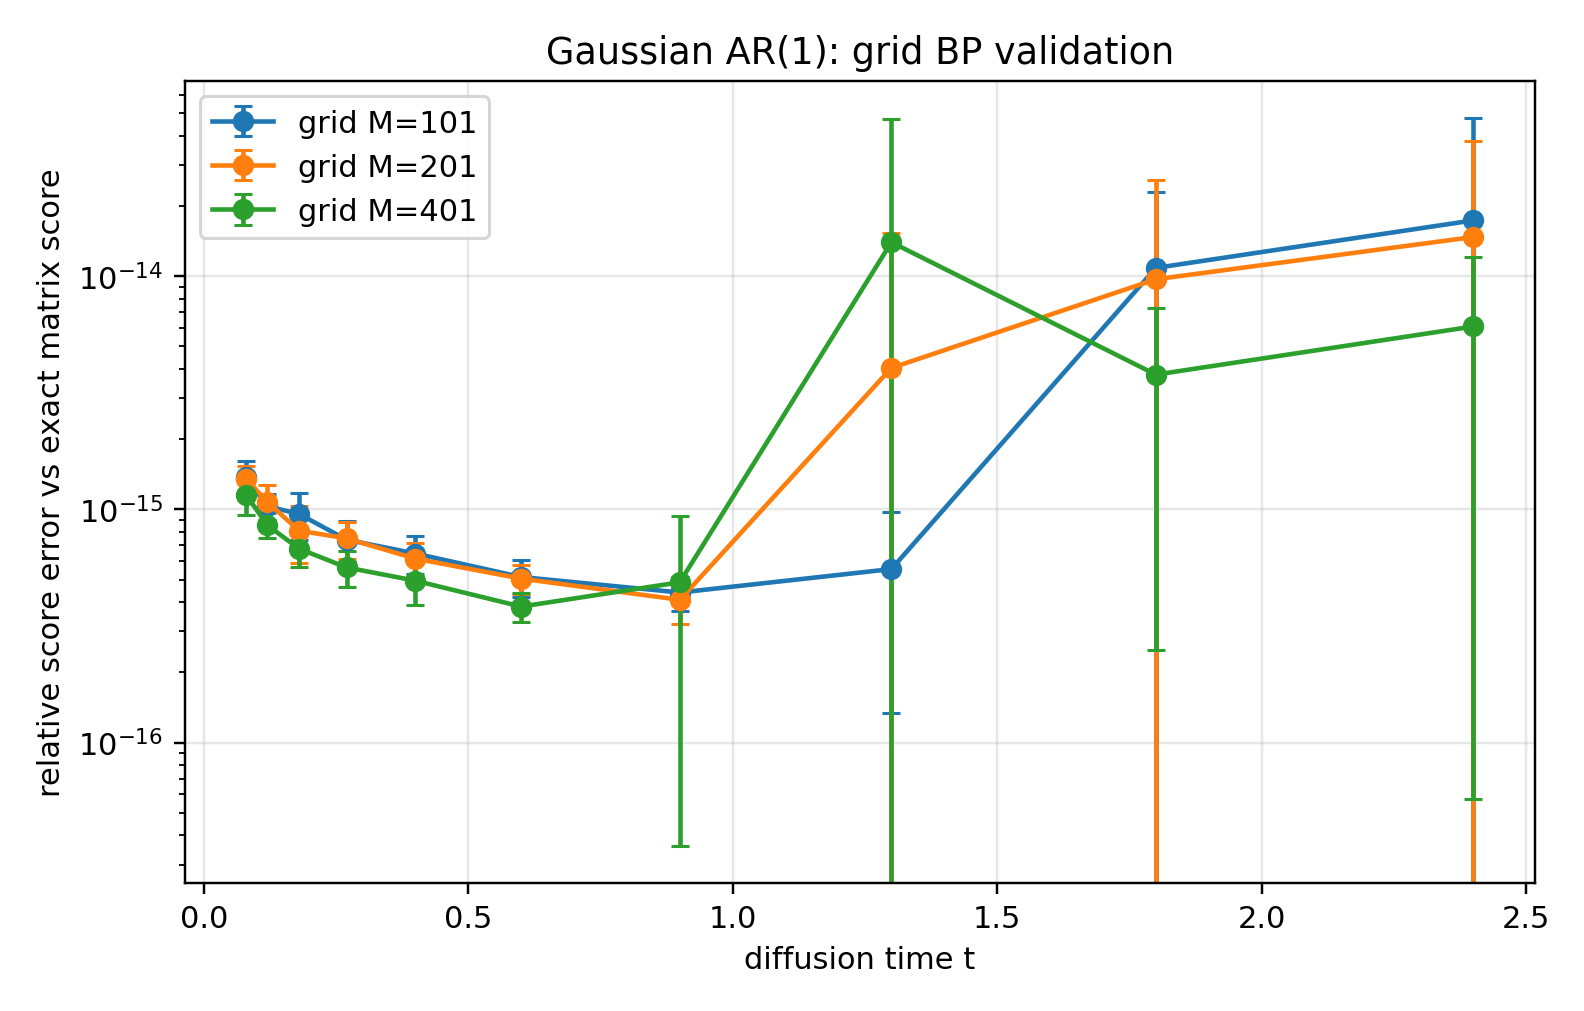
\includegraphics[width=0.88\textwidth]{../outputs/gaussian_grid_validation_rel_error.png}
  \caption{Gaussian AR(1) validation: relative error between grid BP score and exact precision-matrix score. The error is extremely small for the chosen interval and grid sizes, confirming that grid BP is a reliable numerical reference in this controlled case.}
  \label{fig:gaussian-validation}
\end{figure}

Figure \ref{fig:closuresanity} checks Gaussian message closure in the Gaussian case, where
it should be exact. The information-form recursion of Section~\ref{sec:closure} sits at
\(2\times10^{-16}\) uniformly in \(t\), confirming that the Gaussian family really is closed
under the BP updates and that nothing is lost by storing only two scalars per message.

The same figure overlays the discarded grid projection of Section~\ref{sec:ablation}.
Although structurally it makes the same Gaussian assumption, its error grows by fifteen
orders of magnitude across the time range, reaching \(1.8\times10^{-1}\) at \(t=2.4\), and
is essentially independent of \(M\) --- confirming that the failure comes from the width of
the truncation rather than from its resolution.

\begin{figure}[H]
  \centering
  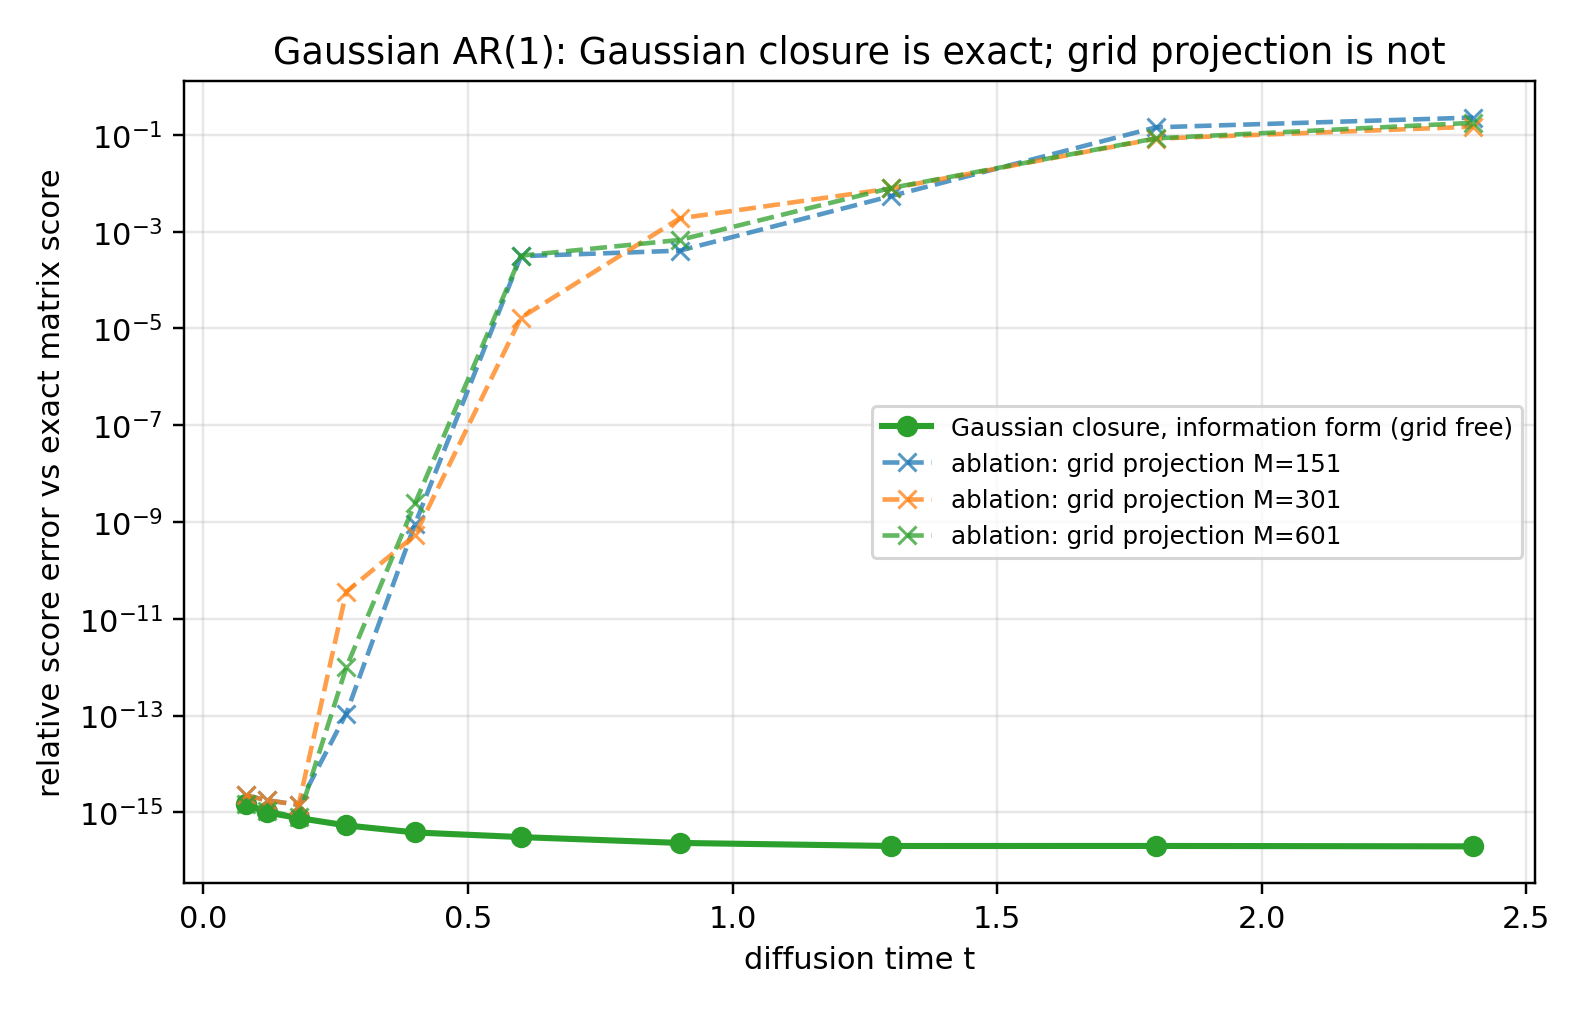
\includegraphics[width=0.88\textwidth]{../outputs/gaussian_closure_sanity_rel_error.png}
  \caption{Gaussian AR(1): Gaussian message closure against the exact matrix score. The
  grid-free information-form recursion (solid) is exact to machine precision at every
  diffusion time. The discarded grid projection (dashed) is shown as an ablation; its
  error grows with \(t\) because \(\alpha_t\to0\) flattens the messages and the moment
  matching then measures the width of the grid rather than the shape of the message. The
  three dashed curves nearly coincide, showing the failure is insensitive to \(M\).}
  \label{fig:closuresanity}
\end{figure}

\subsection{Laplace grid convergence}

In the Laplace case there is no precision-matrix score. Figure \ref{fig:laplace-grid-convergence} compares grid BP with \(M=201\) and \(M=401\). This estimates the grid discretization error of the reference method.

\begin{figure}[H]
  \centering
  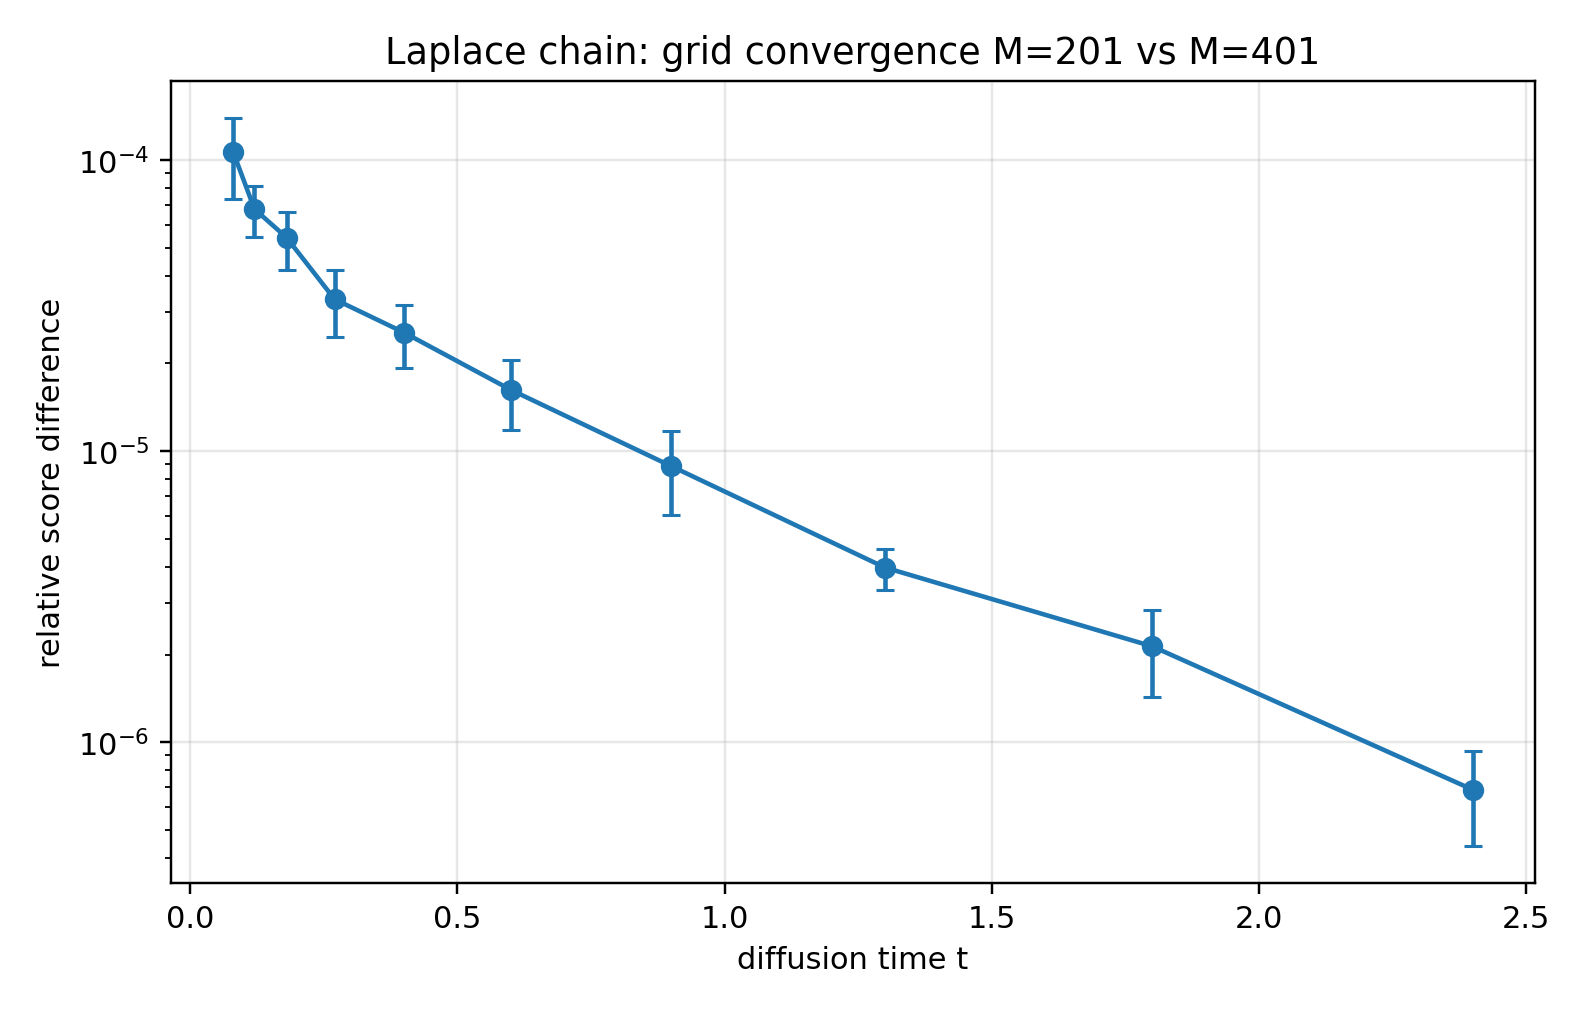
\includegraphics[width=0.88\textwidth]{../outputs/laplace_grid_convergence_rel_error.png}
  \caption{Laplace chain grid convergence: relative score difference between coarse grid \(M=201\) and fine grid \(M=401\). This is our proxy for grid discretization error in the non-Gaussian case.}
  \label{fig:laplace-grid-convergence}
\end{figure}

Representative values from the Laplace grid-convergence CSV are:
\begin{center}
\begin{tabular}{rrrr}
\toprule
\(t\) & Relative score difference & Posterior mean MSE & Score cosine \\
\midrule
0.08 & \(1.25\times 10^{-4}\) & \(1.23\times 10^{-9}\) & 0.99999999 \\
0.40 & \(2.91\times 10^{-5}\) & \(7.92\times 10^{-10}\) & 0.9999999996 \\
1.30 & \(4.48\times 10^{-6}\) & \(2.37\times 10^{-10}\) & 0.99999999999 \\
2.40 & \(7.81\times 10^{-7}\) & \(8.67\times 10^{-11}\) & 1.0000000000 \\
\bottomrule
\end{tabular}
\end{center}

The key interpretation is that the grid-discretization error is much smaller than the Gaussian-message approximation error measured below, at least for the report settings.

\subsection{Gaussian-message approximation error in the Laplace chain}

By Proposition~\ref{prop:lmmse} the Gaussian closure applied to this chain returns exactly
the linear denoiser, so the quantities plotted here are the excess error of the best
linear estimator relative to the exact one. The identity is confirmed numerically: the
relative gap between the closure output and \(\alpha_t\Sigma_0\Sigma_t^{-1}x\) is at most
\(8.5\times10^{-16}\) across the whole time range.

Figure \ref{fig:laplace-mean-mse} shows posterior-mean MSE. Figure \ref{fig:laplace-rel-score} shows relative score error. Figure \ref{fig:laplace-cosine} shows score cosine similarity.

\begin{figure}[H]
  \centering
  
\includegraphics[width=0.88\textwidth]{../outputs/laplace_posterior_mean_mse.png}
  \caption{Laplace chain: posterior-mean MSE between Gaussian message closure and reference grid BP.}
  \label{fig:laplace-mean-mse}
\end{figure}

\begin{figure}[H]
  \centering
  
\includegraphics[width=0.88\textwidth]{../outputs/laplace_relative_score_error.png}
  \caption{Laplace chain: relative score error of Gaussian message closure compared with reference grid BP. The error decreases monotonically with diffusion time: as \(t\) grows the posterior is increasingly dominated by the Gaussian likelihood and the linear estimator becomes correspondingly better. The non-monotonic behaviour reported in the first version of this note was an artefact of the grid projection discussed in Section~\ref{sec:ablation}.}
  \label{fig:laplace-rel-score}
\end{figure}

\begin{figure}[H]
  \centering
  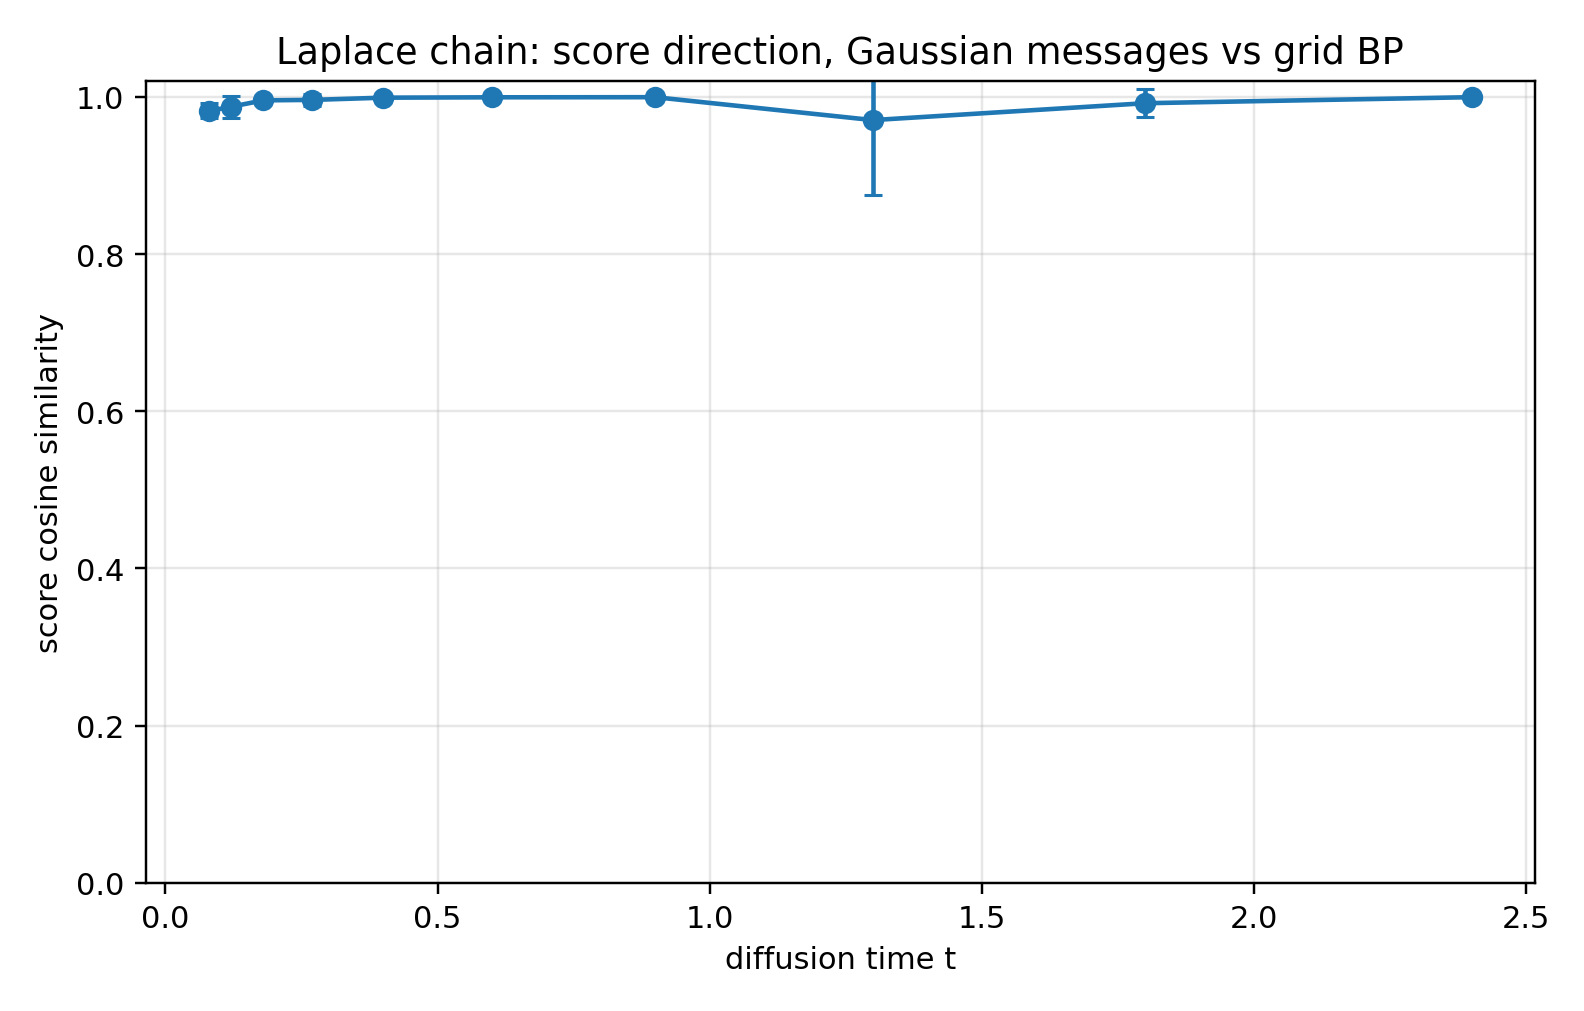
\includegraphics[width=0.88\textwidth]{../outputs/laplace_score_cosine_similarity.png}
  \caption{Laplace chain: cosine similarity between Gaussian-message score and reference grid-BP score. Even when the norm error is non-negligible, the direction remains close at all diffusion times.}
  \label{fig:laplace-cosine}
\end{figure}

Representative values, over 50 trials per time:
\begin{center}
\begin{tabular}{rrrrr}
\toprule
\(t\) & Posterior mean MSE & Relative score error & Score cosine & Closure vs LMMSE \\
\midrule
0.08 & \(3.15\times 10^{-3}\) & 0.199 & 0.9806 & \(8.5\times10^{-16}\) \\
0.12 & \(3.37\times 10^{-3}\) & 0.147 & 0.9887 & \(6.8\times10^{-16}\) \\
0.40 & \(1.94\times 10^{-3}\) & 0.0418 & 0.9990 & \(4.9\times10^{-16}\) \\
0.90 & \(1.66\times 10^{-3}\) & 0.0133 & 0.9999 & \(3.6\times10^{-16}\) \\
1.80 & \(2.07\times 10^{-5}\) & \(7.50\times10^{-4}\) & 1.0000 & \(4.0\times10^{-16}\) \\
2.40 & \(1.03\times 10^{-6}\) & \(8.68\times10^{-5}\) & 1.0000 & \(6.2\times10^{-16}\) \\
\bottomrule
\end{tabular}
\end{center}

Two features of this table are worth recording. First, both error measures now decrease
monotonically in \(t\); the large values previously reported at \(t=1.80\) and \(t=2.40\)
were entirely due to the grid projection. Second, the largest discrepancy occurs at
\emph{small} diffusion times, where the posterior is sharp and the non-Gaussian shape of
the Laplace innovations is least washed out by the observation noise.

It does not follow that small times are the ones that matter for generation. The score
error and the sampling error are different quantities, related by the whole backward
trajectory rather than pointwise, and the accumulated effect of a score error at time
\(t\) is not proportional to its size. Settling this requires running the reverse process
with the exact and approximate scores and comparing the generated distributions; that is
the natural next experiment and it is listed first in Section~\ref{sec:nextsteps}.

\subsection{Example beliefs}

Figure \ref{fig:laplace-belief} compares a posterior belief at one site. This is the most concrete way to see what Gaussian projection does: it replaces the reference grid posterior shape by a Gaussian-message-induced approximation.

\begin{figure}[H]
  \centering
  
\includegraphics[width=0.88\textwidth]{../outputs/example_laplace_belief_comparison.png}
  \caption{Example posterior marginal in the Laplace chain. The reference grid BP belief is compared with the Gaussian closure belief, which by Proposition~\ref{prop:lmmse} is the linear denoiser. The vertical lines show the corresponding posterior means.}
  \label{fig:laplace-belief}
\end{figure}

Figure \ref{fig:gaussian-example} shows an example Gaussian validation score component comparison.

\begin{figure}[H]
  \centering
  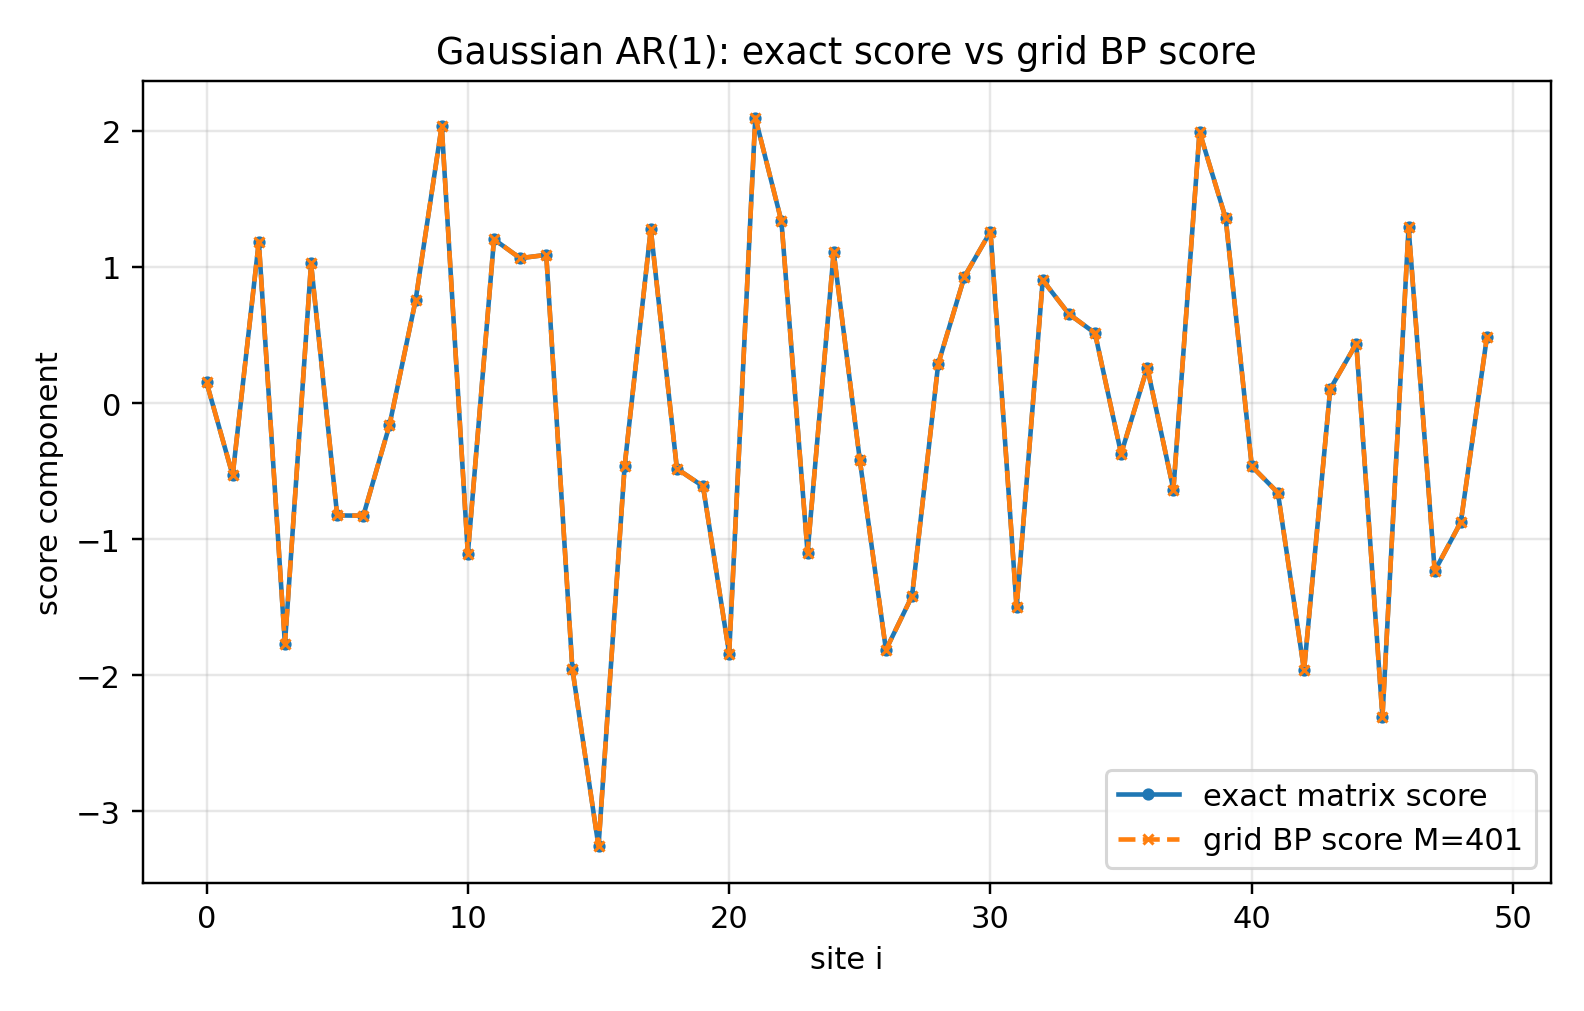
\includegraphics[width=0.88\textwidth]{../outputs/example_gaussian_grid_vs_matrix_score.png}
  \caption{Gaussian AR(1) example: exact precision-matrix score versus grid BP score.}
  \label{fig:gaussian-example}
\end{figure}

\section{Code explanation}

The Python script is
\begin{center}
\texttt{code/bp\_general\_markov\_diffusion\_experiments.py}.
\end{center}
It is organized in layers matching the mathematics.

\subsection{Configuration}

The dataclass \texttt{ExperimentConfig} stores all experimental parameters:
\begin{lstlisting}[style=pythonstyle]
@dataclass
class ExperimentConfig:
    n: int = 50
    rho: float = 0.85
    grid_min: float = -8.0
    grid_max: float = 8.0
    validation_grid_sizes: tuple[int, ...] = (101, 201, 401)
    convergence_coarse_grid_size: int = 201
    ref_grid_size: int = 401
    n_trials: int = 6
    seed: int = 11
    output_dir: str = "bp_markov_diffusion_outputs"
    t_values: tuple[float, ...] = (...)
\end{lstlisting}
This makes it easy to rerun heavier experiments by changing \texttt{n\_trials}, \texttt{ref\_grid\_size}, or the grid interval.

\subsection{Densities and numerical normalization}

The functions \texttt{normal\_pdf} and \texttt{laplace\_pdf} implement the Gaussian and Laplace densities. The function \texttt{trapezoid\_weights} builds quadrature weights. The function \texttt{normalize\_density} normalizes grid values as a density:
\begin{lstlisting}[style=pythonstyle]
def normalize_density(values: np.ndarray, weights: np.ndarray) -> np.ndarray:
    values = np.maximum(np.asarray(values, dtype=float), 0.0)
    mass = float(np.sum(values * weights))
    if not np.isfinite(mass) or mass <= 0.0:
        raise FloatingPointError("Cannot normalize density.")
    return values / mass
\end{lstlisting}
Normalization after each message update is numerically important. BP messages are only defined up to multiplicative constants, so normalization does not change beliefs, but it prevents underflow/overflow over long chains.

\subsection{Transition matrices}

The transition matrix is stored as
\begin{equation}
  K[\text{out},\text{in}]=p(a_{\rm out}\mid a_{\rm in}).
\end{equation}
This convention makes the forward update a matrix-vector product:
\begin{equation}
  L_{i+1}=K\left[(L_i\odot \ell_i)\odot w\right].
\end{equation}
The code is:
\begin{lstlisting}[style=pythonstyle]
def build_transition_matrix(grid, rho, prior):
    q = 1.0 - rho ** 2
    out = grid[:, None]
    inn = grid[None, :]
    if prior == "gaussian":
        return normal_pdf(out, rho * inn, q)
    if prior == "laplace":
        return laplace_pdf(out, rho * inn, np.sqrt(q / 2.0))
\end{lstlisting}

\subsection{Grid BP implementation}

The core of \texttt{grid\_bp} mirrors equations \eqref{eq:grid-forward} and \eqref{eq:grid-backward}:
\begin{lstlisting}[style=pythonstyle]
L[0] = normalize_density(normal_pdf(grid, 0.0, 1.0), weights)
for i in range(n - 1):
    incoming = L[i] * ell[i] * weights
    L[i + 1] = K @ incoming
    L[i + 1] = normalize_density(L[i + 1], weights)

R[-1] = np.ones(m)
for i in range(n - 1, 0, -1):
    incoming = R[i] * ell[i] * weights
    R[i - 1] = K.T @ incoming
    R[i - 1] = normalize_density(R[i - 1], weights)
\end{lstlisting}
After the two passes, beliefs and means are computed as:
\begin{lstlisting}[style=pythonstyle]
b = normalize_density(L[i] * ell[i] * R[i], weights)
means[i] = np.sum(grid * b * weights)
\end{lstlisting}
This is exactly the discrete quadrature version of the exact BP belief formula.

\subsection{Gaussian message closure implementation}

The function \texttt{gaussian\_closure\_bp} takes only \((x,\rho,q,\alpha_t,\Delta_t)\) --- no
grid, no transition matrix --- and propagates the two information scalars directly:
\begin{lstlisting}[style=pythonstyle]
lam_t = lam_L[i] + lam_obs           # multiply by the local likelihood
h_t   = h_L[i]   + h_obs[i]
mu_t, v_t = h_t / lam_t, 1.0 / lam_t
v_out = q + rho ** 2 * v_t           # push through the transition
lam_L[i + 1] = 1.0 / v_out
h_L[i + 1]   = rho * mu_t / v_out
\end{lstlisting}
The flat terminal right message is represented by zero precision, which is the exact
encoding of infinite variance and costs nothing:
\begin{lstlisting}[style=pythonstyle]
lam_R[-1], h_R[-1] = 0.0, 0.0
\end{lstlisting}
Beliefs are then formed by adding information parameters, and the posterior mean is
\(h_i/\lambda_i\).

\subsection{The grid-projection ablation}

\texttt{gaussian\_projected\_bp\_grid} retains the earlier implementation, in which the same
Gaussian assumption is routed through the grid:
\begin{lstlisting}[style=pythonstyle]
L_values = gaussian_message_values(grid, L_mean[i], L_var[i])
incoming = L_values * ell[i] * weights
outgoing = K @ incoming
L_mean[i + 1], L_var[i + 1] = density_moments(outgoing, grid, weights)
\end{lstlisting}
with the flat terminal message written as
\begin{lstlisting}[style=pythonstyle]
R_mean[-1] = 0.0
R_var[-1] = np.inf
\end{lstlisting}
The helper \texttt{gaussian\_message\_values} returns a vector of ones when the variance is
infinite, and \texttt{density\_moments} then assigns that constant the variance of the
truncation interval rather than infinity. This single line is the origin of the failure
analysed in Section~\ref{sec:ablation}.

\subsection{Exact Gaussian score functions}

For validation, the code builds
\begin{equation}
  \Sigma_0(i,j)=\rho^{|i-j|},
  \qquad
  \Sigma_t=\alpha_t^2\Sigma_0+\Delta_t I,
\end{equation}
and computes
\begin{equation}
  s=-\Sigma_t^{-1}x
\end{equation}
using \texttt{np.linalg.solve}:
\begin{lstlisting}[style=pythonstyle]
def gaussian_precision_score(x, rho, alpha, delta):
    sigma0 = ar1_covariance(len(x), rho)
    sigmat = alpha ** 2 * sigma0 + delta * np.eye(len(x))
    return -np.linalg.solve(sigmat, x)
\end{lstlisting}
Using \texttt{solve} is numerically preferable to explicitly computing \(\Sigma_t^{-1}\).

\subsection{Experiment runners}

The script has three experiment runners:
\begin{enumerate}[label=\arabic*.]
  \item \texttt{run\_gaussian\_grid\_validation}: compares grid BP, Gaussian closure and the grid-projection ablation against the exact matrix score.
  \item \texttt{run\_laplace\_grid\_convergence}: compares coarse-grid and fine-grid BP in the Laplace chain.
  \item \texttt{run\_laplace\_gaussian\_message\_error}: compares Gaussian closure against reference grid BP in the Laplace chain, and verifies the LMMSE identity.
\end{enumerate}
The final function \texttt{run\_all} executes all experiments, writes CSV files, and generates plots.

\subsection{How to run}

From the root folder of the delivered archive:
\begin{lstlisting}[style=pythonstyle]
python code/bp_general_markov_diffusion_experiments.py --mode quick
\end{lstlisting}
for a fast smoke test, or
\begin{lstlisting}[style=pythonstyle]
python code/bp_general_markov_diffusion_experiments.py --mode report
\end{lstlisting}
for the report-quality run. To increase experiment weight:
\begin{lstlisting}[style=pythonstyle]
python code/bp_general_markov_diffusion_experiments.py \
    --mode report \
    --n-trials 50 \
    --ref-grid-size 801 \
    --output-dir outputs_heavy
\end{lstlisting}
The cost grows approximately as \(O(nM^2)\), so increasing \(M\) is much more expensive than increasing the number of trials.

\section{Interpretation and next steps}
\label{sec:nextsteps}

The clean conclusion is:
\[
\boxed{\text{BP gives the exact score for Markov-chain priors under OU noising.}}
\]
The hard part is not the score formula. The hard part is continuous message representation.

The Gaussian approximation should therefore be studied as a message-representation approximation. In the Laplace-innovation experiment, the grid error is tiny compared with the Gaussian-message error, so the observed discrepancy primarily reflects Gaussian closure error rather than grid error.

Natural next steps are:
\begin{enumerate}[label=\arabic*.]
  \item Increase trials and grid size to reduce Monte Carlo variability.
  \item Explore different \(\rho\), because stronger correlations make messages more informative and potentially more non-Gaussian.
  \item Compare Laplace, Student, Gaussian-mixture, and bounded-support innovations.
  \item Add Gaussian-mixture message approximations to see how many mixture components are needed to beat single-Gaussian closure.
  \item Study whether neural message approximators help only when they preserve the local BP update structure.
\end{enumerate}

The proposed thesis direction is not that neural networks are unnecessary in general. In real diffusion models, the clean prior \(p_0\) is unknown and must be learned from data. The precise claim is more structural:
\begin{quote}
Score learning can be reformulated as posterior denoising. For Markov-chain priors, posterior denoising is exact BP. When exact continuous BP is not computationally closed, one must approximate the messages. Gaussian messages are the first approximation to test, and their error can be measured directly through the posterior-mean/score identity.
\end{quote}

\appendix
\section{Files in the delivered folder}

The delivered folder contains:
\begin{center}
\begin{tabular}{ll}
\toprule
File & Purpose \\
\midrule
\texttt{report/bp\_markov\_diffusion\_gaussian\_approx.pdf} & this report as PDF \\
\texttt{report/bp\_markov\_diffusion\_gaussian\_approx.tex} & LaTeX source \\
\texttt{code/bp\_general\_markov\_diffusion\_experiments.py} & full experiment script \\
\texttt{code/bp\_general\_markov\_diffusion\_experiments.ipynb} & executable/exploratory notebook \\
\texttt{outputs/*.csv} & numerical experiment tables \\
\texttt{outputs/*.png} & plots used in the report \\
\bottomrule
\end{tabular}
\end{center}

\section{Source references}

\begin{thebibliography}{9}

\bibitem{internalGaussianAR1}
G. Mantovani, \emph{Belief Propagation for the Gaussian AR(1) Diffusion Model: A complete derivation and numerical comparison with the precision-matrix score}, internal project note, 2026.

\bibitem{mezardMontanari}
M. Mezard and A. Montanari, \emph{Information, Physics, and Computation}, Oxford University Press, 2009. Relevant background: factor graphs and belief propagation on trees.

\bibitem{krzakalaZdeborova}
F. Krzakala and L. Zdeborova, \emph{Statistical Physics Methods in Optimization and Machine Learning}, lecture notes, 2024. Relevant background: BP equations, sparse graphs, and the Bethe perspective.

\bibitem{biroliMezardLargeDim}
G. Biroli and M. Mezard, \emph{Generative diffusion in very large dimensions}, arXiv:2306.03518, 2023.

\bibitem{dynamicalRegimes}
G. Biroli, T. Bonnaire, V. de Bortoli, and M. Mezard, \emph{Dynamical Regimes of Diffusion Models}, arXiv:2402.18491, 2024.

\bibitem{unetBP}
S. Mei, \emph{U-Nets as Belief Propagation: Efficient Classification, Denoising, and Diffusion in Generative Hierarchical Models}, arXiv:2404.18444, 2024.

\bibitem{ampBP}
G. Genovese and A. Piana, \emph{Derivation of the AMP Equations from Belief Propagation for the \(\ell_2\) Minimisation Problem}, arXiv:2602.15191, 2026.

\end{thebibliography}

\end{document}
